\subsubsection{User story}
Trong hệ thống được tạo ra vấn đề cốt yếu để tạo ra giá trị cho các đối tượng tham gia chính là việc kết nối người có và người cần homestay lại với nhau. Vậy trong hệ thống này, những thông tin về địa điểm có cho thuê homestay là yếu tố quan trọng nhất. Do đó đối với chủ nhà mà nới thì việc đăng tin là tối cần thiết. Bên cạnh đó, vì tin sẽ được hệ thống duyệt do đó sẽ có khả năng tin mà chủ nhà muốn đăng sẽ không hợp lệ do lý do nào đó. Khi đó người chủ nhà sẽ cần chỉnh sửa lại tin đó sao cho hợp lệ và gửi lại cho hệ thống.Đồng thời người chủ nhà cũng có thể duyệt các tin mà mình đã đăng, đồng thời xóa bỏ nó.

\subsubsection{Mô tả các use case}

\subsubsubsection{Use Case 1: Thêm mới}
\begin{figure}[!h]
	\centering
	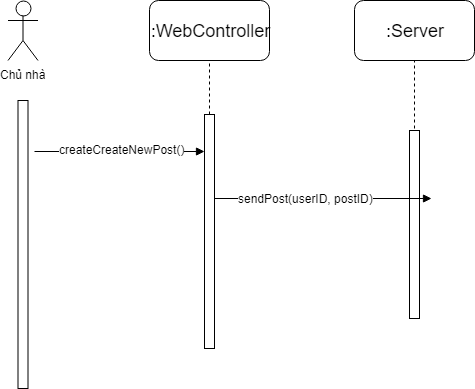
\includegraphics[width=10cm]{parts/bao/images/SequenceDiagram_NewPost.png}
	\caption{Sequence Diagram cho Use Case Thêm mới}
\end{figure}
\begin{center}
	\begin{longtable}{ | l |p{10cm}|}
		\hline
		\textbf{Tên usecase} & Thêm mới \\ \hline
		\textbf{Người tương tác} & Chủ nhà \\ \hline   
		\textbf{Mô tả} &  Người chủ nhà có thể đăng tin về nhu cầu cho thuê homestay của mình. Tin này sẽ được gửi lên hệ thống để chờ duyệt.\\ \hline  
		\textbf{Người tạo:} \textit{Lê Đăng Bảo} & \textbf{Cập nhật lần cuối bởi:} \textit{Văn Tiến Cường} \\ \hline
		\textbf{Ngày tạo:} \textit{30/03/2019} & \textbf{Lần cuối cập nhật:} \textit{30/03/2019} \\ \hline
		\textbf{Tiền điều kiện} &  Người dùng đăng nhập vào hệ thống với vai trò người dùng. \\ \hline 
		\textbf{Hậu điều kiện} &  Thông tin về vị trí thuê được gửi lên server để chờ được duyệt. \\ \hline 
		\textbf{Luồng cơ bản} & 
		\begin{enumerate}
			\item Người dùng chọn tính năng "Đăng tin".
			\item Danh sách các thông tin cần điền hiện ra, người chủ homestay sẽ phải điền đầy đủ thông tin như yêu cầu.
			\item Người dùng chọn "Đăng duyệt".
			\item Hệ thống hiện thông báo về tin đã đăng..
			\item Hệ thống quay lại màn hình chính.
		\end{enumerate} \\ \hline 
		\textbf{Luồng thay thế} & 
		\begin{itemize} 
			\item \textit{Luồng thay thế 1}
			\begin{enumerate}
				\item Tại bước 3, khi người dùng chọn "Duyệt tin" nhưng có một số thông tin còn thiếu trong danh sách thông tin hoặc thông tin không hợp lệ mà có thể kiểm tra ngay lúc đó được (như số điện thoại không hợp lệ) thì hệ thống sẽ gửi thông báo thiếu thông tin và đưa người dùng quay lại danh sách thông tin cần điền.
			\end{enumerate}
		\end{itemize} \\ \hline 
		
		\textbf{Ngoại lệ} &
		\begin{itemize}
		    \item Tại bước 4, khi không có lỗi có thể kiểm tra ngay được nhưng đường truyền mạng của người dùng có vấn đề và khi đó hệ thống sẽ gửi thông báo "Gửi không thành công, kiểm tra lại hệ thống mạng".
		\end{itemize} \\ \hline
	\end{longtable}
\end{center}


\subsubsubsection{Use Case 2: Xem danh sách tin}
\begin{figure}[!h]
	\centering
	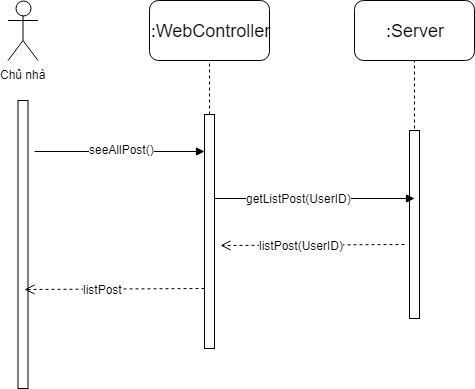
\includegraphics[width=10cm]{parts/bao/images/SequenceDiagram_ListPost.png}
	\caption{Sequence Diagram cho UseCase Xem danh sách tin}
\end{figure}
\begin{center}
	\begin{longtable}{ | l |p{10cm}|}
		\hline
		\textbf{Tên usecase} & Xem danh sách tin \\ \hline
		\textbf{Người tương tác} & Chủ nhà \\ \hline   
		\textbf{Mô tả} &  Người chủ nhà dùng khi muốn xem lại các tin mình đã đăng, để xem lại mình có sai sót gì trong quá trình tạo thông tin hay không.\\ \hline  
		\textbf{Người tạo:} \textit{Lê Đăng Bảo} & \textbf{Cập nhật lần cuối bởi:} \textit{Lê Đăng Bảo} \\ \hline
		\textbf{Ngày tạo:} \textit{30/03/2019} & \textbf{Lần cuối cập nhật:} \textit{30/03/2019} \\ \hline
		\textbf{Tiền điều kiện} &  Người dùng đăng nhập vào hệ thống với vai trò người dùng. \\ \hline 
		\textbf{Hậu điều kiện} &  Danh sách những tin mà người dùng đã đăng lên hệ thống. \\ \hline 
		\textbf{Luồng cơ bản} & 
		\begin{enumerate}
			\item Người dùng chọn tính năng "Danh sách tin đăng".
			\item Yêu cầu sẽ được gửi lên hệ thống và danh sách các tin mà người dùng đã đăng sẽ được trả về.
			\item Người dùng quay lại màn hình chính.
			
		\end{enumerate} \\ \hline 
		\textbf{Luồng thay thế} & 
		\begin{itemize} 
			\item \textit{Luồng thay thế 1}
			\begin{enumerate}
				\item Tại bước 2, Nếu người dùng chưa từng đăng thông tin nào thì thông tin trả về sẽ là rỗng.
			\end{enumerate}

		\end{itemize} \\ \hline 
		\textbf{Ngoại lệ}  & Không có \\
		\hline
	\end{longtable}
\end{center}

\subsubsection{Use Case 3: Chỉnh sửa tin đã đăng}
\begin{figure}[!h]
	\centering
	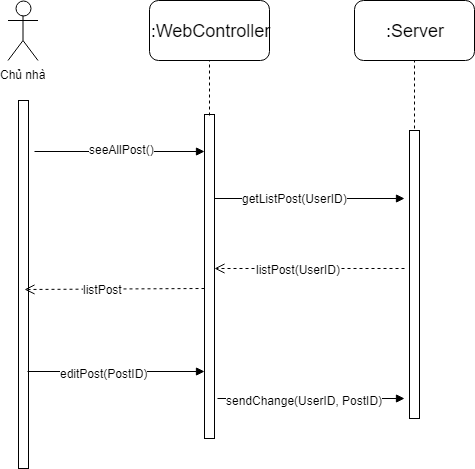
\includegraphics[width=10cm]{parts/bao/images/SequenceDiagram_EditPost.png}
	\caption{Sequence Diagram cho UseCase Chỉnh sửa tin đã đăng}
\end{figure}
\begin{center}
	\begin{longtable}{ | l |p{10cm}|}
		\hline
		\textbf{Tên usecase} & Chỉnh sửa tin đã đăng \\ \hline
		\textbf{Người tương tác} & Chủ nhà \\ \hline   
		\textbf{Mô tả} &  Tin người dùng đăng lên đôi khi vì lý do nào đó, không đáp ứng được những yêu cầu mà hệ thống quy định (như hình ảnh bị trùng, thông tin không hợp lệ) thì tin sẽ không được hệ thống duyệt, trong trường họp đó, thóng báo sẽ được gửi về cho chủ nhà. Trong trường hợp này người dùng phải chỉnh sửa lại thông tin sao cho hợp lệ rồi sẽ được gửi đi để duyệt lại.\\ \hline  
		\textbf{Người tạo:} \textit{Lê Đăng Bảo} & \textbf{Cập nhật lần cuối bởi:} \textit{Lê Đăng Bảo} \\ \hline
		\textbf{Ngày tạo:} \textit{30/03/2019} & \textbf{Lần cuối cập nhật:} \textit{30/03/2019} \\ \hline
		\textbf{Tiền điều kiện} &  Người dùng đăng nhập vào hệ thống với vai trò người dùng và tin sắp được chỉnh sửa phải là tin bị trả về do không hợp lệ. \\ \hline 
		\textbf{Hậu điều kiện} &  Thông tin được gửi lại hệ thống để chờ duyệt. \\ \hline 
		\textbf{Luồng cơ bản} & 
		\begin{enumerate}
			\item Người dùng chọn tính năng "Danh sách tin đăng".
			\item Trong danh sách hiện ra nếu có tin không hợp lệ thì sẽ có màu sắc khác. Người chủ chọn tin đó.
			\item Người dùng chỉnh sửa lại tin theo yêu cầu được gửi về (điểm chưa hợp lệ).
			\item Chọn "Gửi lại" để gửi lại tin đã chỉnh sửa về hệ thống.
			\item Người dùng quay lại màn hình chính.
			
		\end{enumerate} \\ \hline 
		\textbf{Luồng thay thế} & 
		\begin{itemize} 
			\item \textit{Luồng thay thế 1}
			\begin{enumerate}
				\item Tại bước 4, nếu người dùng chỉnh sửa lại thông tin mà có thông tin không hợp lệ được kiểm tra ngay lúc đó (như số điện thoại không đủ số) thì người dùng sẽ được đưa lại phần chỉnh sửa để sửa lại tin.
			\end{enumerate}
		\end{itemize} \\ \hline 
		\textbf{Ngoại lệ}  & 
		\begin{itemize}
		    \item Tại bước 4, nếu đường truyền bị lỗi thì sẽ gửi thông báo cho người dùng và quay trở lại trang chủ.
		\end{itemize} \\ \hline
	\end{longtable}
\end{center}

\subsubsubsection{Use Case 4: Ẩn tin đã đăng}
\begin{figure}[!h]
	\centering
	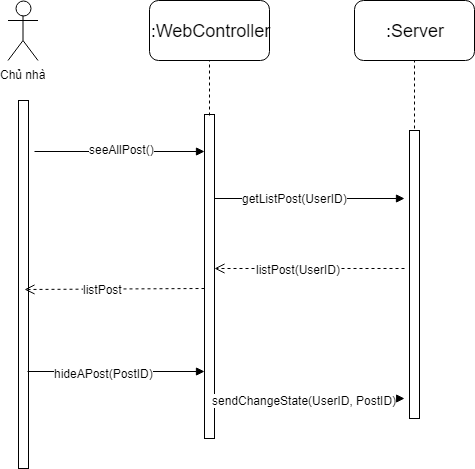
\includegraphics[width=10cm]{parts/bao/images/SequenceDiagram_HidePost.png}
	\caption{Sequence Diagram cho UseCase Ẩn tin đã đăng}
\end{figure}
\begin{center}
	\begin{longtable}{ | l |p{10cm}|}
		\hline
		\textbf{Tên usecase} & Ẩn tin đã đăng \\ \hline
		\textbf{Người tương tác} & Chủ nhà \\ \hline   
		\textbf{Mô tả} &  Khi mà chủ nhà đã tìm được người thuê nhà phù hợp thì chủ nhà có thể ẩn tin đã đăng. Tin được ẩn sẽ được lưu lại chứ không được xóa.\\ \hline  
		\textbf{Người tạo:} \textit{Lê Đăng Bảo} & \textbf{Cập nhật lần cuối bởi:} \textit{Lê Đăng Bảo} \\ \hline
		\textbf{Ngày tạo:} \textit{30/03/2019} & \textbf{Lần cuối cập nhật:} \textit{30/03/2019} \\ \hline
		\textbf{Tiền điều kiện} &  Người dùng đăng nhập với vai trò người dùng. \\ \hline 
		\textbf{Hậu điều kiện} &  Tin được ẩn sẽ được sẽ được gửi lên server để thay đổi dữ liệu trên đó. \\ \hline 
		\textbf{Luồng cơ bản} & 
		\begin{enumerate}
			\item Người dùng chọn tính năng "Danh sách tin đăng".
			\item Chọn tin muốn ẩn. Sẽ vào phần hiển thị thông tin của tin đó.
			\item Người dùng chọn "Ẩn tin" để gửi yêu cầu lên hệ thống.
			\item Người dùng quay lại màn hình chính.
			
		\end{enumerate} \\ \hline 
		\textbf{Luồng thay thế} & Không có \\ \hline
		
		\textbf{Ngoại lệ} &%
		\begin{itemize}
		    \item Tại bước 3, nếu đường truyền bị lỗi thì sẽ gửi thông báo cho người dùng và quay trở lại trang chủ.
		\end{itemize} \\ \hline 
	\end{longtable}
\end{center}